% chktex-file 1
% chktex-file 2
% chktex-file 3
% chktex-file 8
% chktex-file 12
% chktex-file 13
% chktex-file 18
% chktex-file 24
% chktex-file 26
% chktex-file 36
% chktex-file 44
\documentclass[aps,prl,reprint,superscriptaddress,nofootinbib,floatfix]{revtex4-2}

\usepackage[utf8]{inputenc}
\usepackage[T1]{fontenc}
\usepackage{amsmath,amssymb,bm}
\usepackage{graphicx}
\usepackage{booktabs}
\usepackage[final]{microtype}
\usepackage{silence}
\WarningFilter{nameref}{The definition of \label has changed}
\usepackage[colorlinks=true,citecolor=blue,linkcolor=blue,urlcolor=blue]{hyperref}
\Urlmuskip=0mu plus 1mu\relax
\emergencystretch=1em
\hbadness=3000
\makeatletter
\@ifpackageloaded{babel}{}{\let\selectlanguage\@gobble}
\def\@bibdataout@aps{%
 \immediate\write\@bibdataout{%
  @CONTROL{%
   apsrev42Control%
   \longbibliography@sw{%
    ,author="09",editor="0",pages="0",title="0",year="1"%
   }{%
    ,author="09",editor="0",pages="0",title="",year="1"%
   }%
  }%
 }%
 \if@filesw
  \immediate\write\@auxout{\string\citation{apsrev42Control}}%
 \fi
}%
\makeatother

\begin{document}

\title{Mutation-process priors calibrate protein language models for retrospective genotype--phenotype evolutionary ranking}

\author{Hyoseok Jang}
\thanks{These authors contributed equally.}
\affiliation{Computational Science Research Center, Korea Institute of Science and Technology (KIST), Seoul 02792, Republic of Korea}
\affiliation{AI-Robot Department, University of Science and Technology (UST), Seoul 02792, Republic of Korea}
\author{Sangchul Lee}
\thanks{These authors contributed equally.}
\affiliation{Computational Science Research Center, Korea Institute of Science and Technology (KIST), Seoul 02792, Republic of Korea}
\author{David S. Yang}
\thanks{These authors contributed equally.}
\affiliation{Chemical and Biological Integrative Research Center, Korea Institute of Science and Technology, Seoul 02792, Republic of Korea}
\author{Haneol Cho}
\affiliation{Computer Science and Engineering, Sejong University, Seoul 05006, Republic of Korea}
\author{Cherlhyun Jeong}
\email{che.jeong@kist.re.kr}
\affiliation{Chemical and Biological Integrative Research Center, Korea Institute of Science and Technology, Seoul 02792, Republic of Korea}
\affiliation{Division of Bio-Medical Science \& Technology, University of Science and Technology, Seoul 02792, Republic of Korea}
\author{Chansoo Kim}
\email{eau@ust.ac.kr}
\affiliation{Computational Science Research Center, Korea Institute of Science and Technology (KIST), Seoul 02792, Republic of Korea}
\affiliation{AI-Robot Department, University of Science and Technology (UST), Seoul 02792, Republic of Korea}

\date{}

\begin{abstract}
PLMs score amino-acid substitutions in protein space, but evolution samples nucleotide changes in genotype space. We introduce codon-aware constrained semantic change (CAC), a post-hoc calibration that adds a codon-transition prior from a nucleotide Markov process to PLM scores, requiring no retraining. In a retrospective SARS-CoV-2 Spike benchmark, CAC improves recovery of deep-mutational-scanning antibody-escape annotations, reducing ESM-2-3B mean rank from $9130$ to $5037$. Tuning the Markov horizon reveals a crossover from mutational accessibility to protein-level constraints.
\end{abstract}

\maketitle

\emph{Introduction.--}
Protein language models (PLMs) score amino-acid substitutions for mutation effects, fitness, and annotated immune-escape phenotypes \cite{Riesselman2018,Rives2021,Meier2021,hie2021learning,lin2023evolutionary}. Constrained semantic change search (CSCS) ranks substitutions by combining semantic change in representation space with grammaticality, the probability or pseudolikelihood that the substituted sequence remains compatible with learned protein constraints \cite{hie2021learning}.

For evolutionary interpretation, protein-space ranking omits the process that supplies variants. Natural variation is sampled as stochastic nucleotide changes, translated through the genetic code, and then filtered by selection. This mapping is uneven: substitutions with comparable PLM scores can differ strongly in codon accessibility or nucleotide bias \cite{Halpern1998,Rodrigue2010,Duffy2018mutation}. Retrospective evolutionary ranking therefore needs both a protein-level score and a genotype-level accessibility term.

This gives a calibration problem rather than a forecasting problem. Mutation-selection models make the same separation: mutation supplies an unequal distribution of variants, and selection acts on their phenotypic consequences \cite{Halpern1998,Rodrigue2010}. We test whether the same separation improves black-box PLM rankings.

Here we implement codon-aware constrained semantic change (CAC): a model-agnostic reweighting of CSCS by a codon-transition prior inferred from observed single-base substitution spectra \cite{Yi2021Mutational}. The prior is a continuous-time nucleotide Markov process projected through the genetic code to amino-acid accessibility. Because CAC only reorders an existing substitution list, it applies to specialized PLMs and frozen foundation models without retraining. Backbone-independent gains would expose a shared calibration gap between amino-acid scoring and nucleotide sampling. We therefore ask whether codon accessibility improves retrospective recovery of published phenotype annotations and how that contribution changes with the dimensionless Markov horizon.

\begin{figure}[tbp]
    \centering
    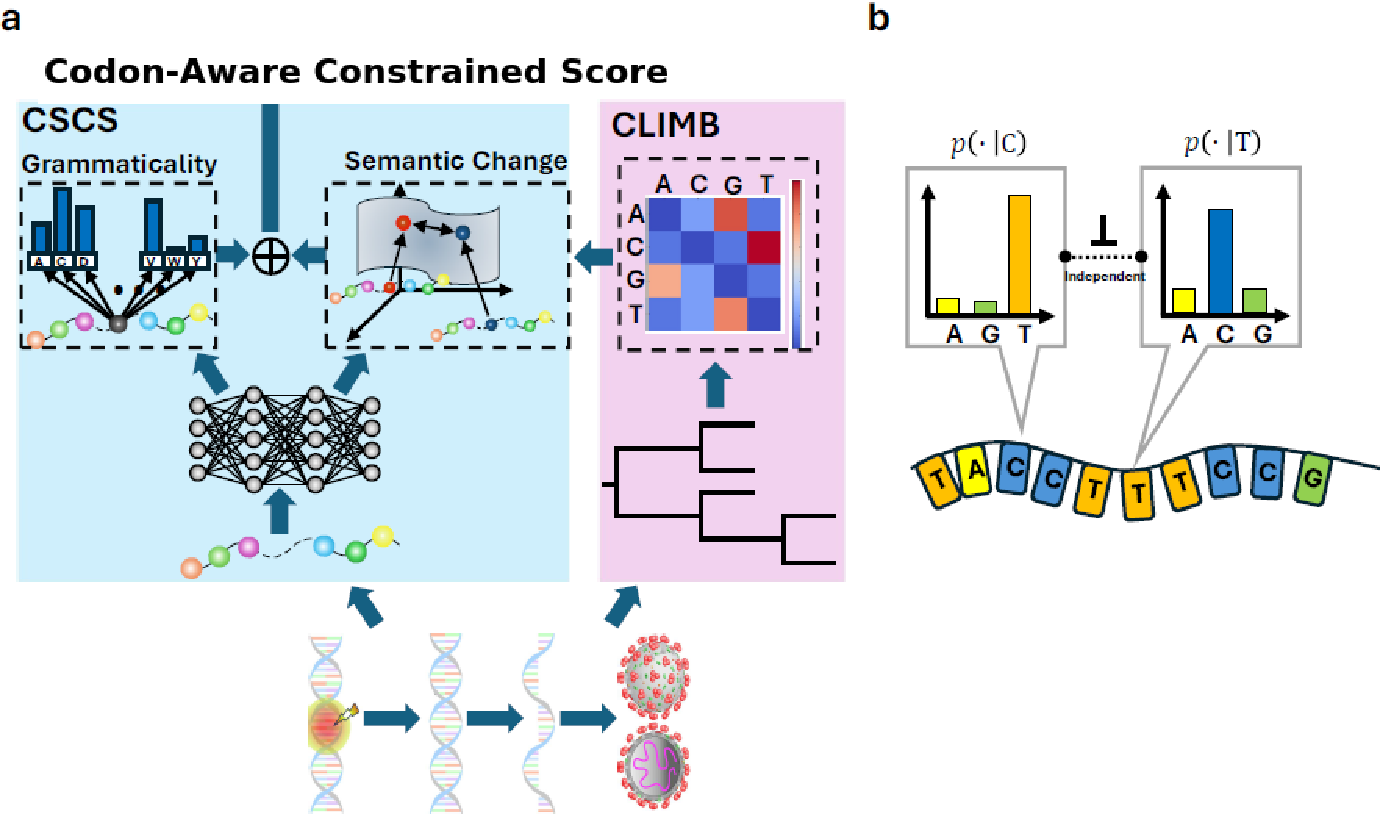
\includegraphics[width=\linewidth]{fig1.pdf}
    \caption{\textbf{Process-aware calibration of protein language models.}
    A PLM scores candidate amino-acid substitutions by semantic change $s_{\rm s}$, measured from distances between learned sequence embeddings, and grammaticality $s_{\rm g}$, measured from model probability or pseudolikelihood. CAC augments this amino-acid objective with a codon-accessibility term $s_{\rm p}=\log p_T$ computed from a nucleotide continuous-time Markov process. Empirical substitution spectra estimate the nucleotide generator $Q$; the genetic code maps this process to unequal probabilities for amino-acid substitutions. The calibration therefore reweights PLM rankings toward substitutions that are both protein-compatible and genetically accessible.}
    \label{fig:framework}
\end{figure}

\emph{Codon-transition prior.--}
The prior is a nucleotide transition process projected through the genetic code \cite{Halpern1998,Rodrigue2010}. For RNA alphabet $\mathcal{B}=\{\mathsf{A},\mathsf{C},\mathsf{G},\mathsf{U}\}$ and generator $Q=(q_{uv})_{u,v\in\mathcal{B}}$, base transitions over dimensionless horizon $T$ have probabilities $[\exp(TQ)]_{uv}$. The horizon $T$ controls neighborhood breadth rather than calendar time. With independent codon positions, the probability that wild-type codon $\bm c=(c_1,c_2,c_3)$ produces amino acid $\tilde a$ is
\begin{equation}
    p_T(\tilde a \mid \bm c)
    =
    \sum_{\tilde{\bm c}:\,g(\tilde{\bm c})=\tilde a}
    \prod_{k=1}^{3}
    [\exp(TQ)]_{c_k \tilde c_k},
    \label{eq:codon-prior}
\end{equation}
where $g$ maps codons to amino acids. We estimate $Q$ from published SARS-CoV-2 substitution counts by normalizing empirical transition fluxes with base frequencies; details, the matrix, and a context-dependence check are in the Supplemental Material.

For each candidate substitution, CAC combines this codon-likelihood Markov-bias accessibility term (CLIMB) with semantic change and grammaticality,
\begin{equation}
\begin{split}
    S_{\rm CAC}
    =
    \alpha z(s_{\rm s})
    + \beta z(\log s_{\rm g})
    + \gamma z(\log p_T),
    \\
    \alpha+\beta+\gamma=1,
    \label{eq:cac}
\end{split}
\end{equation}
where $z(\cdot)$ standardizes over all nonsynonymous single-nucleotide substitutions of the reference Spike sequence. Setting $\gamma=0$ gives CSCS; positive $\gamma$ adds CLIMB to the same candidates, changing only their ranks.

\emph{Retrospective phenotype ranking.--}
We evaluated all $24\,187$ nonsynonymous single-nucleotide substitutions of SARS-CoV-2 Wuhan-Hu-1 Spike. Protein scores came from Hie-BiLSTM \cite{hie2021learning} and ESM-2-150M, ESM-2-650M, and ESM-2-3B \cite{lin2023evolutionary}. Validation used published deep mutational scanning (DMS) antibody-escape measurements \cite{baum2020antibody} and characteristic substitutions from major lineages. Performance was the mean rank of these annotations; lower ranks indicate earlier retrospective recovery.

\begin{figure}[tbp]
    \centering
    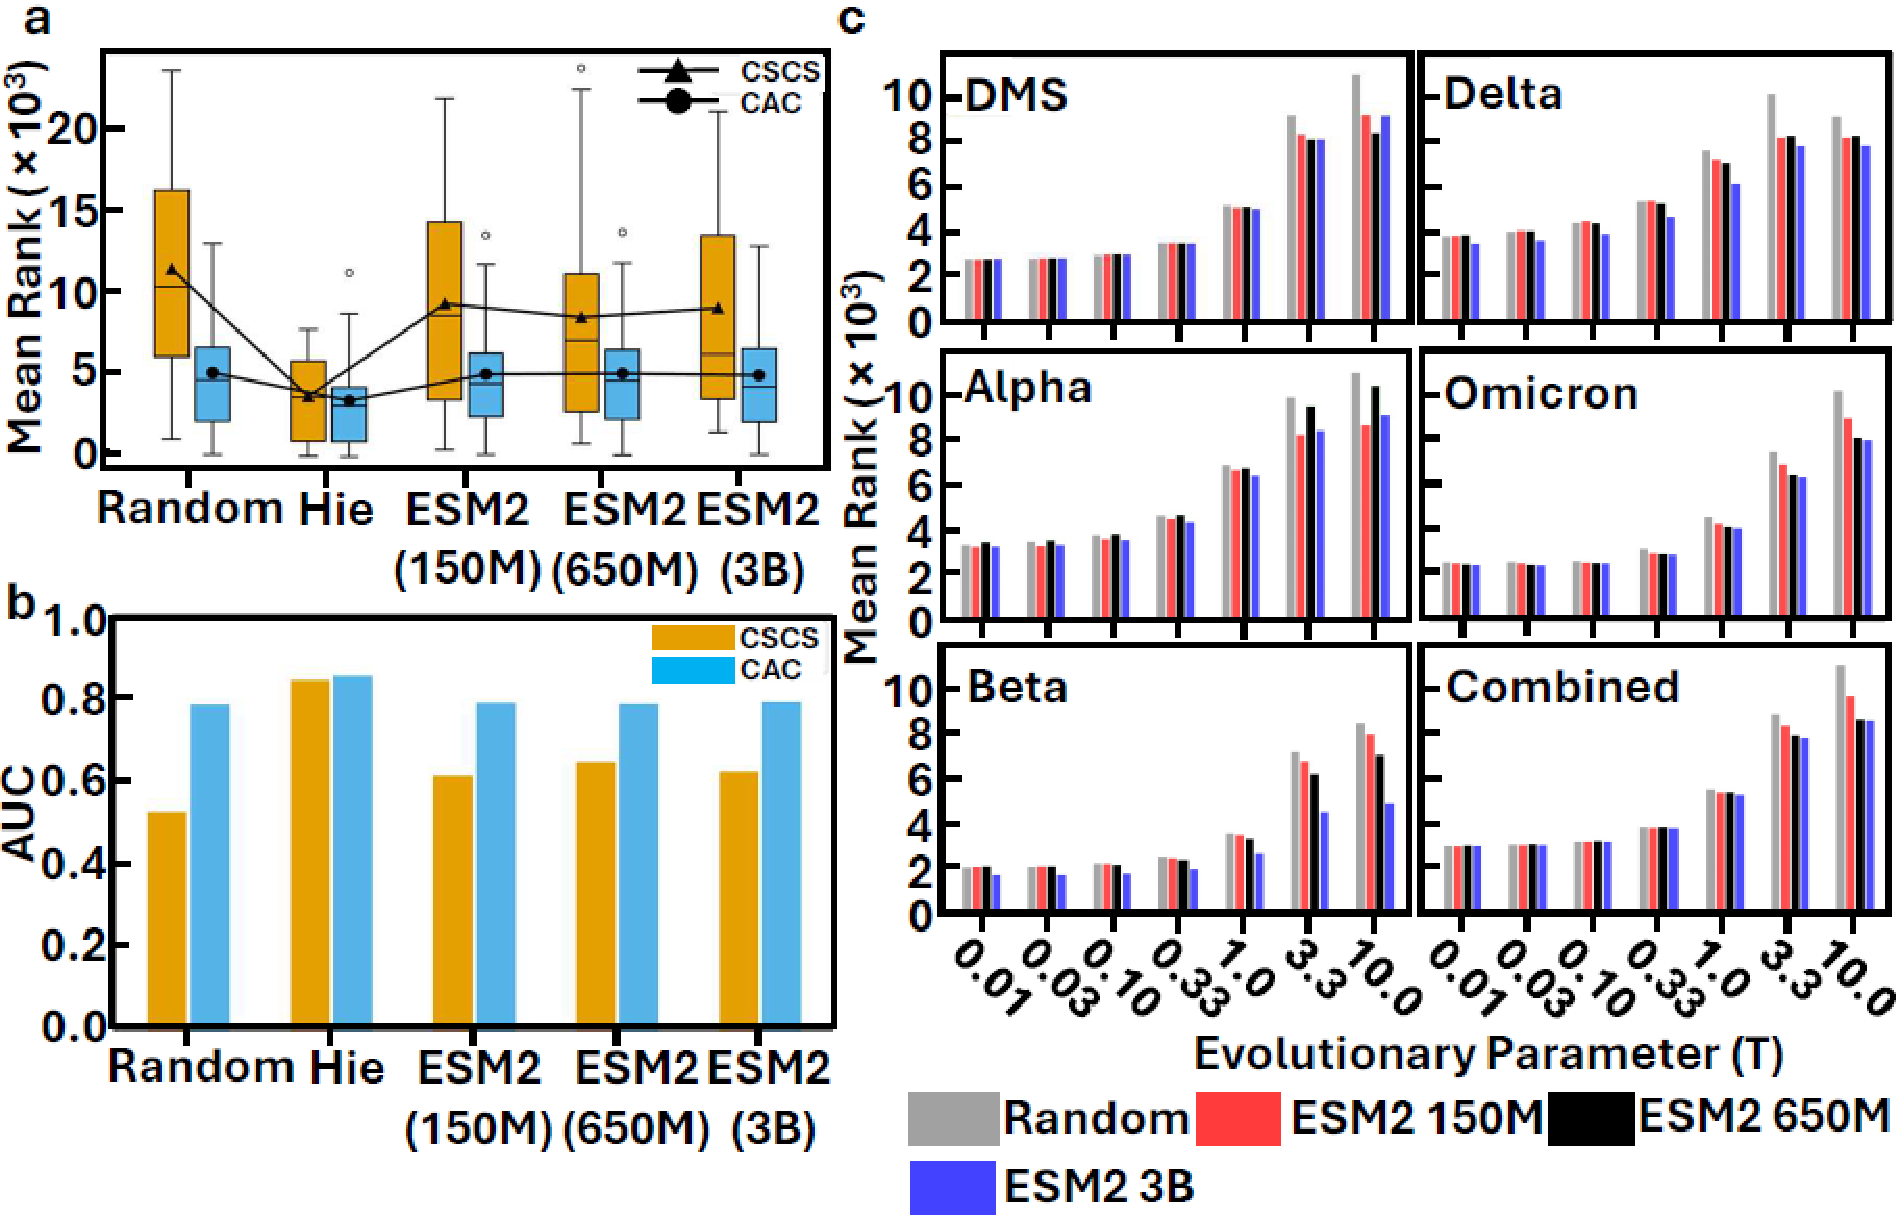
\includegraphics[width=\linewidth]{fig2.pdf}
    \caption{\textbf{Codon-aware calibration improves retrospective recovery of annotated phenotypes.}
    CAC is compared with the amino-acid-only CSCS baseline, a CLIMB-only ablation in which protein scores are randomized, and a random baseline. (a) On the DMS antibody-escape annotation set, CAC substantially lowers ranks for general-purpose ESM-2 models. (b) CAC also improves AUC across model backbones. (c) The dependence on dimensionless Markov horizon $T$ shows that local-neighborhood rankings benefit most from the mutation-accessibility prior.}
    \label{fig:performance}
\end{figure}

The codon-transition prior improved retrospective ranking across PLM backbones and validation sets (Fig.~\ref{fig:performance}). On DMS, CAC reduced the ESM-2-3B mean annotation rank from $9130\pm6500$ to $5037\pm3586$ (mean $\pm$ s.d.; one-sided Wilcoxon signed-rank test, $p=0.0031$). It improved ESM-2-150M from $9387\pm6127$ to $5098\pm3667$ and ESM-2-650M from $8562\pm6870$ to $5143\pm3701$. Hie-BiLSTM changed less on DMS, $3757\pm2574$ to $3493\pm2974$, consistent with related evolutionary training data already encoding part of the short-horizon mutational structure.

The combined set of 60 DMS and lineage-associated substitutions gave the same result. CAC lowered the mean rank for Hie-BiLSTM from $6260$ to $3841$, for ESM-2-150M from $9816$ to $5309$, for ESM-2-650M from $8857$ to $5327$, and for ESM-2-3B from $8736$ to $5204$. Full tables, AUC values, and validation-set definitions are in the Supplemental Material. A CLIMB-only ablation achieved a DMS mean rank of $5100\pm184$ across 100 randomizations of the PLM-derived terms, far below the random baseline of $12012\pm1588$. Thus, benchmark annotations carry strong genotype-space structure, while PLM terms add protein-level information on top of this accessibility signal.

\begin{figure}[tbp]
    \centering
    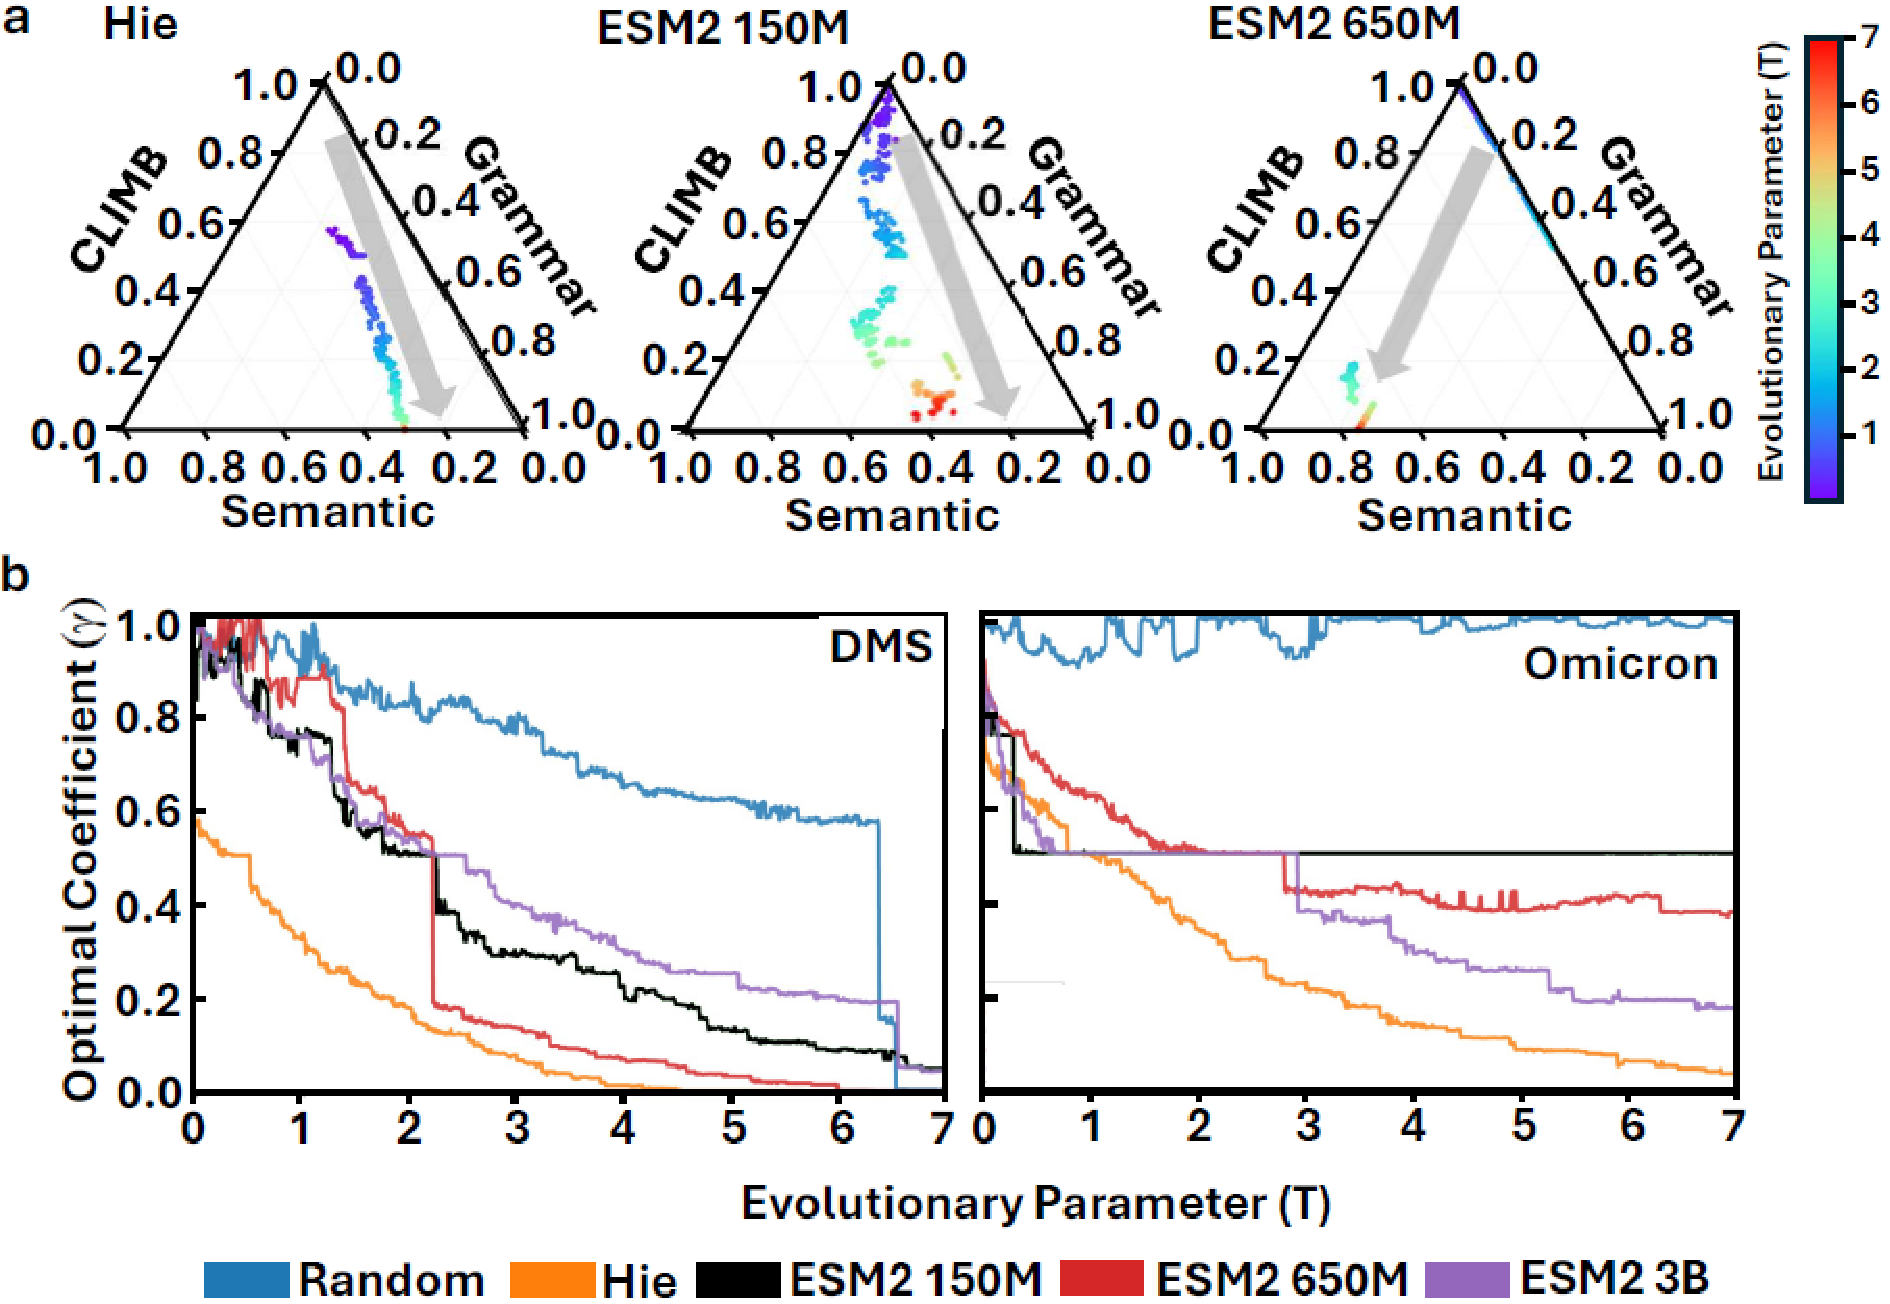
\includegraphics[width=\linewidth]{fig3.pdf}
    \caption{\textbf{Evolutionary horizon controls the mixture of process and protein information.}
    Optimized weights $(\alpha,\beta,\gamma)$ shift systematically with the dimensionless Markov horizon $T$. At small $T$, the CLIMB weight $\gamma$ is large, reflecting strong local mutational accessibility. As $T$ increases, $\gamma$ decreases and the PLM-derived semantic and grammatical terms carry more weight, while the accessibility prior remains active.}
    \label{fig:horizon}
\end{figure}

\emph{Horizon-dependent crossover.--}
The Markov horizon $T$ controls how sharply the prior favors local codon changes. At small $T$, high-probability single-base paths dominate; at larger $T$, probability mass spreads and accessibility becomes less restrictive. Optimizing the simplex weights in Eq.~\eqref{eq:cac} revealed a crossover between these regimes (Fig.~\ref{fig:horizon}). For Hie-BiLSTM on DMS, the optimal CLIMB weight fell from $\gamma=0.5372$ at $T=0.1$ to $\gamma=0.0652$ at $T=3$. Across backbones, small-$T$ rankings were driven mainly by codon accessibility, whereas broader-horizon rankings shifted toward semantic change and grammaticality.

This crossover separates supply from constraint. Local neighborhoods are dominated by the nucleotide process; broader neighborhoods allow more codon paths, making protein compatibility or antigenic change more decisive. CAC exposes this accessibility--constraint tradeoff as an explicit weight rather than burying it in a black-box predictor.

\emph{Discussion.--}
CAC improved retrospective phenotype ranking by adding the missing genotype-space supply term to protein-space PLM scores. The effect was largest for general-purpose ESM-2 models, indicating that codon accessibility is not reliably captured by amino-acid representations alone.

This role is complementary to genomic or temporal models. With sufficient aligned genomes and timestamps, sequence-level models can learn mutation, sampling history, and selection jointly. CAC instead calibrates already computed phenotype-oriented PLM scores, making it portable across backbones and directly testable against future genomic baselines.

The limitations are equally direct. The benchmarks are retrospective; prospective claims require strict held-out time-split evaluations. The prior is minimal, assuming independent sites and context-averaged substitution spectra, but the same form can accommodate context-dependent nucleotide models, lineage-specific spectra, multi-step paths, and epistatic protein constraints. The analysis provides no experimental protocol, variant-construction recommendation, or operational forecast. It shows that PLM rankings become sharper when calibrated to the stochastic process that generates the genotypes selection can see.

\begin{acknowledgments}
This work is supported by grant Nos. 2023-00262155 (AIDE), 2024-00460980 (deFAI), and 2025-02304717 ((AI)$^2$) from IITP; 2025R1A5A1031234 and 2021R1A2C1095046 from NRF; and RS-2023-00266133 from the Korea Health Technology R\&D Project, all funded by the Korean government. We also acknowledge institutional support from KIST. Source code and data are available at \url{https://github.com/sos440/climb} and archived on Zenodo at \url{https://doi.org/10.5281/zenodo.15744443}.
\end{acknowledgments}

\bibliography{sn-bibliography}

\end{document}
